% arara: pdflatex
% arara: pdflatex
% arara: pdflatex


% options:
% thesis=B bachelor's thesis
% thesis=M master's thesis
% czech thesis in Czech language
% english thesis in English language
% hidelinks remove colour boxes around hyperlinks

\documentclass[thesis=M,english]{FITthesis}[2019/12/23]

\usepackage[utf8]{inputenc} % LaTeX source encoded as UTF-8

% \usepackage{subfig} %subfigures
% \usepackage{amsmath} %advanced maths
% \usepackage{amssymb} %additional math symbols

\usepackage{dirtree} %directory tree visualisation

\usepackage{listings}
\lstset{basicstyle=\ttfamily, language=C++}

\usepackage{amsmath}
\usepackage{tabularx}
\usepackage{xcolor}
\usepackage{minted}
\usepackage{algorithm}
\usepackage{algpseudocode}
% TODO: reenable minted if possible.
\usepackage{minted}
\usepackage{amsthm,amssymb,amsfonts}
\usepackage{tikz,lipsum,lmodern}
\usepackage[most]{tcolorbox}
\usepackage{multicol}

% % list of acronyms
% \usepackage[acronym,nonumberlist,toc,numberedsection=autolabel]{glossaries}
% \iflanguage{czech}{\renewcommand*{\acronymname}{Seznam pou{\v z}it{\' y}ch zkratek}}{}
% \makeglossaries

% % % % % % % % % % % % % % % % % % % % % % % % % % % % % % 
% EDIT THIS
% % % % % % % % % % % % % % % % % % % % % % % % % % % % % % 

\department{Department of Theoretical Computer Science}
\title{Distrubuted Sparse Matrix-Vector Multiplication}
\authorGN{Boris} %author's given name/names
\authorFN{Rúra} %author's surname
\author{Boris Rúra} %author's name without academic degrees
\authorWithDegrees{Bc. Boris Rúra} %author's name with academic degrees
\supervisor{doc. Ing. Ivan Šimeček, Ph.D.}
\acknowledgements{TODO: make thanks}
\abstractEN{Summarize the contents and contribution of your work in a few sentences in English language.}
\abstractCS{V n{\v e}kolika v{\v e}t{\' a}ch shr{\v n}te obsah a p{\v r}{\' i}nos t{\' e}to pr{\' a}ce v {\v c}esk{\' e}m jazyce.}
\placeForDeclarationOfAuthenticity{Prague}
\keywordsCS{Replace with comma-separated list of keywords in Czech.}
\keywordsEN{Replace with comma-separated list of keywords in English.}
\declarationOfAuthenticityOption{1} %select as appropriate, according to the desired license (integer 1-6)
% \website{http://site.example/thesis} %optional thesis URL



\newtcolorbox{boxyyy}[2][]{sidebyside,
    lower separated=false,
    righthand ratio=0.56, % to define right-hand fraction
    colback=white,
    colframe=white!20!gray,fonttitle=\bfseries,
    colbacktitle=white!10!gray,enhanced,
    attach boxed title to top left={xshift=1cm,
            yshift=-2mm},
    title=#2,#1}

\newcommand*{\captionsource}[2]{%
    \caption[{#1}]{%
        #1%
        \\\hspace{\linewidth}%
        \textbf{Source:} #2%
    }%
}


\begin{document}

\tableofcontents
% \newacronym{CVUT}{{\v C}VUT}{{\v C}esk{\' e} vysok{\' e} u{\v c}en{\' i} technick{\' e} v Praze}
% \newacronym{FIT}{FIT}{Fakulta informa{\v c}n{\' i}ch technologi{\' i}}

\setsecnumdepth{part}
\chapter{Introduction}

\setsecnumdepth{all}

\chapter{Sparse matrix storage formats}

% TODO: chapter summary

\section{Sparse matrices}

A matrix is a rectangular array of numbers. The numbers in the array
are called the entries in the matrix. \cite{anton14} Matrix entries are usually addressed
by the column and row in the rectangle they occupy.

In numerical analysis and scientific computing, a sparse matrix or sparse array
is a matrix in which most of the elements are zero. There is no strict definition
regarding the proportion of zero-value elements for a matrix to qualify as sparse
but a common criterion is that the number of non-zero elements is roughly equal
to the number of rows or columns. By contrast, if most of the elements are non-zero,
the matrix is considered dense.
The number of zero-valued elements divided by the total number of elements (e.g., m × n for an m × n matrix) is sometimes referred to as the sparsity of the matrix.
\cite{efficientSDMM} The number of non zero elements of a sparse matrix is usually denoted
as $n_{nz}$ number of columns as $n$ and number of rows as $m$.

To better illustrate the storage formats, let us define sparse matrix $A$.
\begin{equation*}
    A =
    \begin{pmatrix}
        1 & 0 & 2 & 0 \\
        0 & 3 & 0 & 0 \\
        4 & 0 & 5 & 0 \\
        6 & 0 & 0 & 7
    \end{pmatrix}
\end{equation*}

\section{Coordinate (COO)}

Coordinate storage format, commonly referred to as COO.
The data structure consists of three arrays of length $n_{nz}$\cite{saad03:IMS}:

% TODO: this may be nicer if formated with minted or something similar.
\begin{enumerate}
    \itemsep=0em
    \item[vals] a real array containing all the real (or complex) values of the nonzero elements of A in any order.
    \item[row\_idx] an integer array containing their row indices.
    \item[col\_idx] a second integer array containing their column indices.
\end{enumerate}

Thus $A$ would be stored as:

\begin{table}[h!]
    \centering
    \begin{tabular}{ |l||c|c|c|c|c|c|c| }
        \hline
        vals     & 1 & 2 & 3 & 4 & 5 & 6 & 7 \\
        \hline
        row\_idx & 0 & 0 & 1 & 2 & 2 & 3 & 3 \\
        \hline
        col\_idx & 0 & 2 & 1 & 0 & 2 & 0 & 3 \\
        \hline
    \end{tabular}
    \caption{$A$ stored in COO format}
\end{table}


\section{Compressed Sparse Row (CSR)}

Compressed Sparse Row is probably the most popular format for storing general sparse matrices.
\cite{saad03:IMS} Similarly to the coordinate format, it too consists of three arrays.

% TODO: better lstinline.
\begin{enumerate}
    \itemsep=0em
    \item[vals] a real array of size $n_{nz}$ containing all the real (or complex) values of the nonzero elements of $A$
        stored in row major order.
    \item[col\_idx] a second integer array of size $n_{nz}$ containing their column indices.
    \item[row\_ptr] an integer array of size $m + 1$ containing offsets into \lstinline{vals} and
        \lstinline!col_idx!, at which each row of the matrix begins.
\end{enumerate}

This involves nonnegligible savings in storage.

\begin{table}[h!]
    \centering
    \begin{tabular}{ |l||c|c|c|c|c|c|c| }
        \hline
        vals     & 1 & 2 & 3 & 4 & 5 & 6 & 7 \\
        \hline
        col\_idx & 0 & 2 & 1 & 0 & 2 & 0 & 3 \\
        \hline
    \end{tabular} \\
    \begin{tabular}{ |l||c|c|c|c|c| }
        \hline
        row\_ptr & 0 & 2 & 3 & 5 & 6 \\
        \hline
    \end{tabular}
    \caption{$A$ stored in CSR format}
\end{table}

\section{Compressed Sparse Row 5 (CSR5)}

\newcommand{\csre}[1]{\mintinline{C++}!#1!}

To achieve near-optimal load balance for matrices with any sparsity structures,
all nonzero entries are partitioned to multiple 2D tiles of the same size.
The CSR5 format has two tuning parameters: $\omega$ and $\sigma$, where $\omega$
is a tile’s width and $\sigma$ is its height. \cite{liu2015csr5}

Further, extra information is needed to efficiently compute
SpMV. For each tile, a tile pointer \csre{tile_ptr} and a tile descriptor \csre{tile_desc} are introduced.
Meanwhile, the three arrays, i.e., row pointer \csre{row_ptr}, column index \csre{col_idx} and value val,
of the classic CSR format are directly integrated. The only difference is that the \csre{col_idx} data and the \csre{vals}
data in each complete tile are in-place transposed (i.e., from row-major order to column-major order) for coalesced memory access from contiguous SIMD lanes.

\textbf{Each column of a tile has three characteristics}:
\begin{itemize}
    \item \csre{y_offset} - relative offset into the Y for a column of tile (equal to number of rows that started in previous columns).
    \item \csre{scansum_offset} - number of consecutive empty columns to the right of current column.
    \item \csre{bit_flag} - of size $\sigma$ where $i-th$ bit is set if $i-th$ value of this column is the first non-0 entry of its row
          or it is the $0th$ bit of $0th$ column.
          %TODO: this could be explained a bit better. 
\end{itemize}

The tile further may have an \csre{empty_offset} array of size $\mathcal{O}(\omega * \sigma)$, if it contains empty rows,
because \csre{y_offset} will be incorrect for such tile. Thus we store correct offsets into Y for each segment of such
a tile in \csre{empty_offset}. The actual size of this array is number of segments in a tile (the number of bits set to 1 in \csre{bit_flag}).

% TODO: remake this, don't use picture.
\begin{figure}[htp]
    \centering
    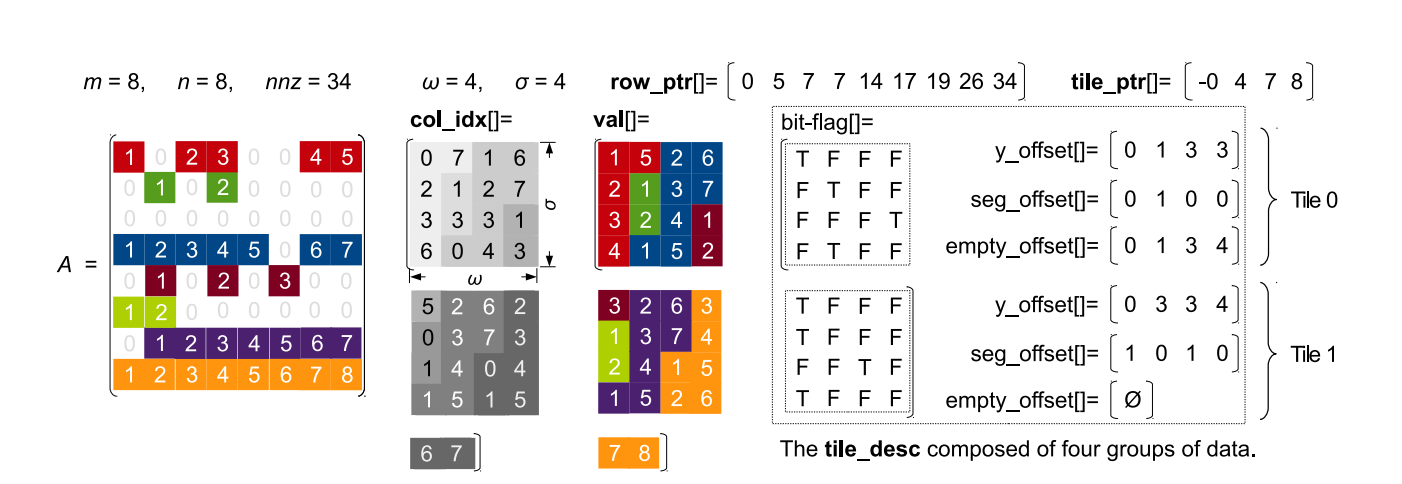
\includegraphics[scale=0.35]{static/csr5_do_not_use_remake.png}
    \caption{Matrix A stored in CSR5 format}
\end{figure}

\chapter{Theory}

% TODO

\section{OpenMP}

OpenMP API is defined by a collection of compiler directives, library routines, and environment variables.
It provides a model for parallel programming that is portable across architectures
from different vendors. Compilers from numerous vendors support the OpenMP API. \cite{openmp18}


\section{MPI}

MPI (Message-Passing Interface) is a message-passing library interface specification.
All parts of this definition are significant. MPI addresses primarily the message-passing parallel
programming model, in which data is moved from the address space of one process to
that of another process through cooperative operations on each process. Extensions to the
“classical” message-passing model are provided in collective operations, remote-memory
access operations, dynamic process creation, and parallel I/O. MPI is a specification, not
an implementation; there are multiple implementations of MPI. This specification is for a
library interface; MPI is not a language, and all MPI operations are expressed as functions,
subroutines, or methods, according to the appropriate language bindings which, for C and
Fortran, are part of the MPI standard.
\cite{mpi40}


\section{SIMD}

As defined in Flynn's taxonomy, Single Instruction Multiple Data (or SIMD) is a type of parallel
processing, where a single instruction is applied to multiple data streams.

Modern CPUs provide Streaming SIMD Extensions (or SSE) Instruction Set Extensions, as well as
Advanced Vector Extensions (or AVX). These can be leveraged in C++ by using OpenMP pragma
directives or compiler provided set of intrinsics.



\section{Sparse matrix exchange formats}


\subsection{Matrix Market Exchange Format}

Native exchange format of Matrix Market. Has two flavours, Array Format for dense matrices,
Coordinate format for sparse matrices. \cite{mmef}

% TODO: citations

\subsubsection{General Format Specification}

All Matrix Market echange format files contain three sections, which must appear in order:

\begin{enumerate}
    \item \textbf{Header} First line of a file, must follow the template:
          \begin{lstlisting}
    %%MatrixMarket object format [qualifier...]
\end{lstlisting}
          Where object type indicates the mathematical object (e.g. vector, matrix) which is
          stored in the file. Type indicates the format (array or coordinate) used to store
          the object. Qualifiers are used to further indicate special properties of the stored
          object (e.g. symmetry, field) thus their number as well as allowed values depend on
          the stored object.
    \item \textbf{Comments} Zero or more line of comments\footnote{Comments are lines starting with \%.}.
    \item \textbf{Data} Remainder of the file contains data representing the object.
          The format of data is dependent on the stored object but for simplicity,
          each data entry should occupy a single line.
\end{enumerate}

\subsubsection{Coordinate Format for Sparse Matrices}

Header format for sparse matrices:
\begin{lstlisting}
%%MatrixMarket matirx coordinate <field> <symmetry>
\end{lstlisting}

% TODO: citation
Where\footnote{For further explanation see the specification.}:
\begin{itemize}
    \item \textbf{field} determines the type and number of values listed for each entry
          and is one of: Real, Complex, Integer or Pattern.
    \item \textbf{symmetry} determines how to interpret matrix entries
          and is one of: General, Symmetric, Skew-Symmetric or Hermitian.
\end{itemize}

While data specification is:
\begin{lstlisting}
    M N L
    I J A(I, J)
    I J A(I, J)
    ...
\end{lstlisting}

First line of data contains exactly three integers:
\begin{itemize}
    \item \csre{M} - number of rows.
    \item \csre{N} - number of columns.
    \item \csre{L} - number of non-zero entries that follows.
\end{itemize}

The following \csre{L} lines each contain \csre{I} - the row index, \csre{J} - the column index
and the corresponding value. Indices are 1 based. Entries not explicitly provided are considered
to be zero, except for those known by symmetry.


\section{HDF5}

HDF5 is a data model, library, and file format for storing and managing data.
It supports an unlimited variety of datatypes, and is designed for flexible and
efficient I/O and for high volume and complex data. HDF5 is portable and is extensible,
allowing applications to evolve in their use of HDF5. The HDF5 Technology suite includes
tools and applications for managing, manipulating, viewing, and analyzing data in the HDF5 format.
\cite{hdf5} HDF5 is defined by HDF5 File Format Specification, which specifies bit-level organization of an HDF5.

\subsection{HDF5 Abstract Data Model}

The HDF5 data model defines building blocks for data organization and specification in HDF5.
It's two primary objects are \textbf{groups} and \textbf{datasets}.

\subsubsection{Group}

HDF5 groups organize data. Every file contains at least a root group.
Each group can contain other groups or be linked to objects in other files.

\begin{figure}[!h]
    \centering
    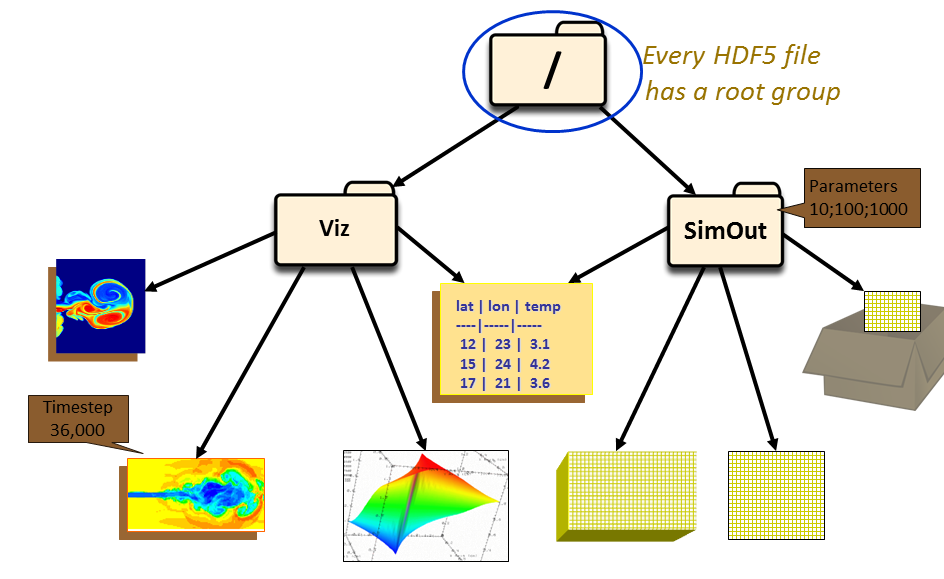
\includegraphics[scale=0.3]{static/group.png}
    % TODO: attribute the picture to HDF5 manual.
\end{figure}

Working with groups and their members is similar to working with files and directories in UNIX.
Objects are often described by giving their path names (e.g. \texttt{/Viz}).

\subsubsection{Dataset}

Datasets organize and contain the "raw" data. They consist of raw data and metadata needed to describe it.
The metadata needed to describe a dataset consists of datatypes, dataspaces, properties and optionally,
attributes.

\begin{figure}[H]
    \centering
    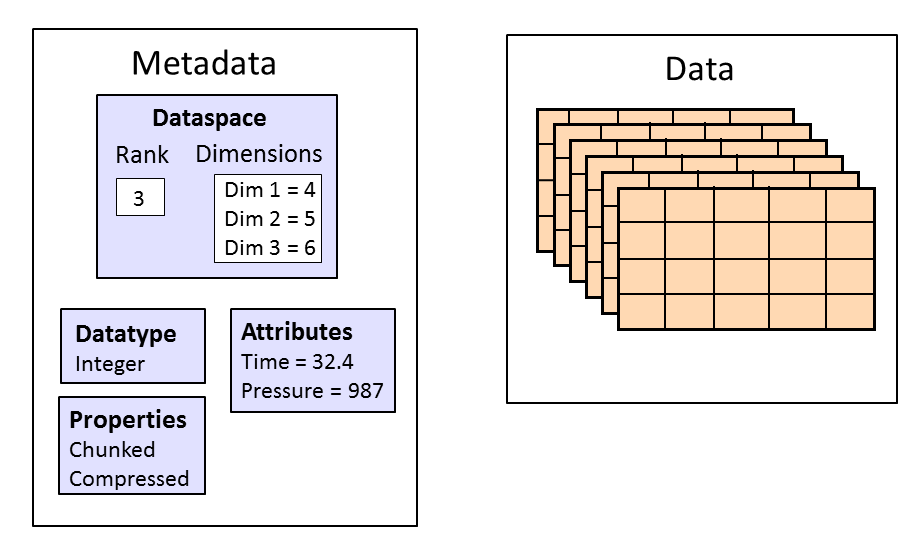
\includegraphics[scale=0.3]{static/dataset.png}
    % TODO: attribute the picture to HDF5 manual.
\end{figure}

\subsubsection{Datatype}

Datatypes describe individual elements in dataset. There are two groups of datatypes:
\begin{itemize}
    \item \textbf{pre-defined} - created by HDF5, contain standard datatypes that are stable across platforms
          (e.g IEEE-754 encoded floating point), as well as native datatypes (e.g. \texttt{double} on platform
          on which the application is running).
    \item \textbf{derived} - created or derived from pre-defined datatypes (e.g. a string).
\end{itemize}

\subsubsection{Dataspace}

Dataspaces describe the layout of datasets elements. It may be empty (NULL), contain a single element (scalar)
or an array\footnote{Number of dimmensions of the array is reffered to as rank of the dataspace.}. They provide
logical layout of a dataset stored in a file (including rank and dimensions). As well as application's data buffers
and data elements participating in I/O. Thus an application can select subsets of a dataset.
% TODO: reference the chapter which will discuss hyperslabs more in depth.

\begin{figure}[H]
    \centering
    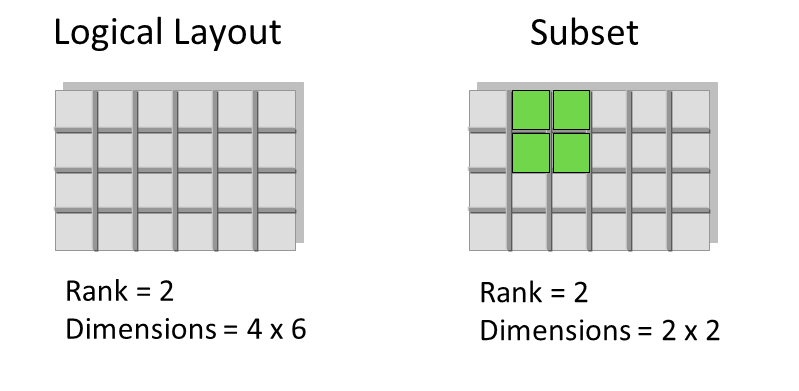
\includegraphics[scale=0.3]{static/dataspace.png}
    % TODO: add source
\end{figure}



\subsubsection{Attribute}

Attributes may optionally be associated with objects. An attribute consists of a name-value pair.
They are similar to datasets in that they too, have a datatype and dataspace. However they do not
support partial I/O, can't be compressed nor extended.





\section{C++20 - TBD}


\chapter{Implementation}

\section{Storage format}

A common issue of distributed SpMV is load balancing. Storing matrices in CSR5 format avoids this by
grouping data into tiles of fixed size. Furthermore the tiles are independent, allowing for high
degree of paralelism.

\subsection{In memory layout}

The three arrays present in CSR \csre{row_ptr}, \csre{col_idx} and \csre{vals} as well as \csre{tile_ptr}
stored in a sequential container (\csre{std::vector} with a custom cache alligned allocator),
while being in-place transformed.

\begin{figure}[!h]
    \begin{minted}{C++}
    struct csr5_t {
        // same as CSR
        uint32_t             num_cols;
        vector<FloatingType> vals;
        vector<uint32_t>     col_idx;
        vector<uint32_t>     row_ptr;
        // CSR5
        vector<uint32_t>     tile_ptr;
        vector<descriptor_t> tile_desc; // shown later.
        vector<uint32_t>     empty_offset_ptr;
        vector<uint32_t>     empty_offset;
    };
    \end{minted}
    \caption{Pseudocode for structure holding CSR5 matrix}
\end{figure}


\subsubsection{Tile descriptor}

Previous research about CSR5 \cite{liu2015csr5} concluded, that for modern CPUs with AVX2 extensions, the optimal CSR5 tuning parameters
are $\sigma = 16$ and $\omega = 4$. Leveraging bit fields, data for each column of tile descriptor may be
stored as:

\begin{minted}{C++}
    struct descriptor_column_t {
        uint32_t y_offset: 7;
        uint32_t scansum_offset: 3;
        uint32_t bit_flag: 16;
    };

    struct descriptor_t {
        descriptor_column_t columns[4];
    };
\end{minted}

Using Non Type Template Parameters, the bit field widths as well as needed underlying type for column
descriptor may be computed at compilation time, allowing for fine-tuning while giving compiler enough
information to optimize properly. This means only 4B additional data per column or 32B per tile.

\subsubsection{Empty offset}

With \csre{empty_offset} being dependent on number of sections in a tile (and being completely absent
in tiles which don't contain empty rows), it would be inefficient to
store it in the descriptor itself. To avoid too many allocations, two supporting arrays are added.
An \csre{empty_offset_ptr} of size $num\_tiles + 1$, which contains offsets for each tile into the
second array, \csre{empty_offset} at which their \csre{empty_offset} array begins.
Thus for each tile, it's empty offset is defined as \csre{empty_offset[empty_offset_ptr[i]:empty_offset_ptr[i+1]]}.


\section{Selecting on disk storage format}


\subsection{Matrix market storage format}

Matrix market exchange format is designed to be easy to parse. It provides a library to parse
the header and matrix dimensions. \cite{mmC}

The numerical entries, need to be parsed manually.
Most implementations use variations of \texttt{scanf}.
Initial implementation in dim used \texttt{scanf} as well. This however proved to be a bottleneck as
the average throughput was only 4515017 elements/s.  After profiling, it beacame obvious that parsing the string representation
was the issue as 97.89\% of time spent was in \texttt{scanf} itself.
To improve the loading times, in an effort to
simplify (and speed up) the process of benchmarking, an implementation using
\mintinline{C++}{scnlib} \footnote{\mintinline{C++}{scnlib} is a modern C++ alternative to scanf.}
was deployed. With an average throughput of 6068194 elements/s it provided about 1.34x speedup but it was still inadequate.

\begin{figure}[!h]
    \centering
    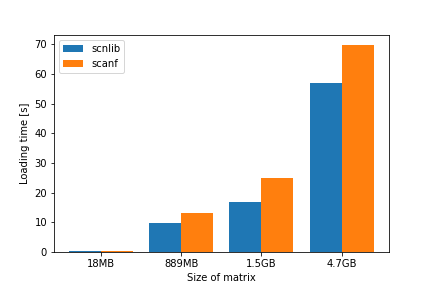
\includegraphics[scale=0.5]{static/MMEF_bench.png}
    \caption{Loading times of MMEF}
\end{figure}

% TODO: maybe cite matlab and PETSc.
\subsection{Matlab compatible HDF5 sparse matrix storage}

\colorlet{hdtsc}{red!60!yellow}
\colorlet{hdatc}{green!60!gray}
\newcommand{\hdts}[1]{\textcolor{hdtsc}{#1}}
\newcommand{\hdat}[1]{\textcolor{hdatc}{#1}}

HDF5 is supported by MATLAB, as well as PETSc. Sparse matrices are stored in CSR format.
Each matrix is represented as a single group containing 3 datasets:
\begin{itemize}
    \item \hdts{data} - values of elements.
    \item \hdts{aj} - column index.
    \item \hdts{ir} - row pointer.
\end{itemize}
And a single attribute \hdat{MATLAB\_sparse} containing number of columns
of the stored matrix.

\newtcolorbox{infobox}[1][]{%
    enhanced,
    left=2pt,
    nobeforeafter,
    width=0.2\textwidth,
    colback={white!30!yellow},
    box align=center,
    baseline=3.5mm,
    colframe=black,
    #1
}

\begin{figure}[!h]
    \begin{tcolorbox}[title=/A, colback=gray!30!white]
        \begin{infobox}[colback=hdtsc]
            data
        \end{infobox}
        \begin{infobox}[colback=hdtsc]
            aj
        \end{infobox}
        \begin{infobox}[colback=hdtsc]
            ir
        \end{infobox}
        \begin{infobox}[colback=hdatc, width=0.35\textwidth]
            MATLAB\_Sparse
        \end{infobox}
    \end{tcolorbox}
    \caption{Layout of a sparse matrix stored as a HDF5 group}
\end{figure}

Storing in this format yielded a throughput of 110005843 elements/s which is 24.36x speedup over \texttt{scanf}
based implementation of reading matrices stored in Matrix Market Echange Format and 18.12x speedup over \texttt{scnlib}
implementation.

\begin{figure}[!h]
    \centering
    \begin{minipage}{.5\textwidth}
        \centering
        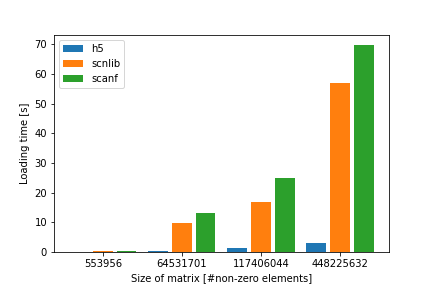
\includegraphics[scale=0.45]{static/matrix_loading.png}
    \end{minipage}%
    \begin{minipage}{.5\textwidth}
        \centering
        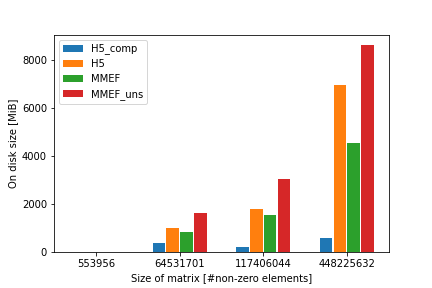
\includegraphics[scale=0.45]{static/storage_sizes.png}
    \end{minipage}
\end{figure}


Since, MMEF uses coordinate format to store sparse matrices, it may ommit elements from symmetrical matrices which can be inferred
from their symmetrical counterparts. This can be used as size optimization. Matrices 2, 3 and 4 in the above graph are symmetrical,
thus their on-disk size can be smaller with MMEF than it is with HDF5.

HDF5 format supports dataset compression by LZMA. Setting chunk size to 4096 and compression level to 5 for each of the 3 datasets,
it is possible to achieve considerable storage savings (the biggest matrix is around 7.8x smaller stored as compressed HDF5 compared to MMEF)
while maintaning better loading performance, with average throughput being 27074837 elements/s, about 4x slower than HDF5 with no compression,
but still 4 and 6 times faster than scnlib and scanf implementations respectively.




\chapter{On disk storage for CSR5 matrices}

HDF5 supports loading only a part of dataset as a hyperslab, making it possible to load only the data
required by a tile to be loaded.




\section{On disk layout}


Each of the sequential data members \hdts{row\_ptr}, \hdts{col\_idx}, \hdts{vals}, \hdts{tile\_ptr},
\hdts{empty\_offset}, \hdts{empty\_offset\_ptr}, are stored as one dimensional datasets of same name
and same datatype. \hdat{num\_cols} is stored as an attribute.

\hdts{tile\_desc} is stored as an one dimensional dataset, with datatype being
an array of 4 little endian unsigned 32-bit integers. In essence storing the data to HDF5 file as
they appear in memory. This does put a soft requirement on the CLI used to transform a CSR matrix to
CSR5 matrix and the code executing the SpMV being compiled by the same version of a compiler, as
bit field in-memory layout is implementation defined, but allows faster loading. Furthermore both
Clang and GCC implement this in the same way so the requirement is only a soft one, as compatibility can
be easily tested.

\begin{figure}[!h]
    \begin{tcolorbox}[title=/A, colback=gray!30!white]
        \begin{infobox}[colback=hdtsc]
            vals
        \end{infobox}
        \begin{infobox}[colback=hdtsc]
            row\_ptr
        \end{infobox}
        \begin{infobox}[colback=hdtsc]
            col\_idx
        \end{infobox}
        \begin{infobox}[colback=hdtsc, width=0.3\textwidth]
            empty\_offset\_ptr
        \end{infobox}
        \begin{infobox}[colback=hdtsc]
            tile\_ptr
        \end{infobox}
        \begin{infobox}[colback=hdtsc]
            empty\_offset
        \end{infobox}
        \begin{infobox}[colback=hdtsc]
            tile\_desc
        \end{infobox}
        \begin{infobox}[colback=hdatc, width=0.2\textwidth]
            num\_cols
        \end{infobox}
    \end{tcolorbox}
    \caption{Layout of a sparse matrix stored as a HDF5 group}
\end{figure}



\section{Loading the matrices}


Since CSR5 partitions the non-zero elements of a matrix into tiles of 
size $\sigma * \omega$, each node can load only data relevant for tiles
assigned to it. This is enabled by two features of HDF5, first of which 
is reading hyperslabs. A hyperslab is a subset of a HDF5 dataset, so 
nodes do not have to read whole datasets. 

Second feature enabling this, is HDF5s ability to utilize MPI-IO, allowing concurrent 
reads from every node rather than reading the matrix in main node 
and distributing it amongst the rest of the nodes. This imposes a minor limitation
on how the matrix can be stored, or rather how the dataset needs to be structured.
Since MPI-IO was introduced in MPI revision 2.0 \cite{mpi20} in 1997, its API takes 
size to be read as an integer argument, thus limiting the maximum amount of data read 
in a single call to 2GiB. The dataset thus needs to be chunked 
\footnote{experimentally, chunks of 1000000 elements or ~8MiB of double precision floating 
point numbers performed best}, else HDF5 tries to read it at once and MPI-IO fails.


To load part of a CSR5 matrix first the number of tiles needs to be obtained. This can be 
done by querying size of \csre{tile_desc} dataset which contains descriptor for each tile.
The number of tiles is then divided by number of nodes, meaning every node gets equal 
number of tiles (bar the last node which can have less) which in turns means equal number 
of non-zero elements.



\begin{algorithm}
    \caption{Computing partition size for each node}
    \begin{algorithmic}
        \Function{calculate\_partition}{$tile\_count$, $node\_id$, $node\_count$}
        \State $partition\_size \gets \lceil\frac{tile\_count}{node\_count}\rceil$
        \State $first \gets partition\_size * node\_id$
        \State $count \gets min(partition\_size, tile\_count - first)$

        \Return $(first, count)$
        \EndFunction
    \end{algorithmic}
\end{algorithm}

Then, tile descriptors from \csre{tile_desc} dataset, tile pointers from \csre{tile_ptr}
dataset and empty offsets pointers from \csre{tile_desc_offset_ptr} can be loaded.
Sizes of slabs are $\#tiles_{node}$, $\#tiles_{node} + 1$ and $\#tiles_{node} + 1$
respectively, as $*\_ptr$ datasets use $n+1^{st}$ element to denote end of values 
belonging to $n^{th}$ element. Lastly empty offsets from \csre{tile_desc_offset} 
are loaded. This forms complete information about CSR5 tiles, and as such, it is 
stored in a separate structure named \csre{csr5_info}. This information is useful 
even on its own, for example queries about a certain tile, matrix element or row 
of matrix and its parent tile can be made just with this information.

\begin{algorithm}
    \caption{Loading CSR5 info}
    \begin{algorithmic}
        \Function{load\_csr5\_info}{$datasets$, $first$, $count$}
        \State $tile\_desc \gets datasets["tile\_desc"][first:first + count]$
        \State $tile\_ptr \gets datasets["tile\_ptr"][first:first + count + 1]$
        \State $empty\_off\_ptr \gets datasets["tile\_desc\_offset\_ptr"][first:first + count + 1]$
        \State $empty\_off \gets datasets["tile\_desc\_offset"][empty\_off\_ptr[0]:empty\_off\_ptr[-1]]$
        \EndFunction
    \end{algorithmic}
\end{algorithm}

\pagebreak

Lastly, slab of \csre{row_ptr} is loaded, starting at \csre{tile_ptr[0]} and 
ending at last output row of chunk of this matrix. This varies, if it is the last 
node, the last output row is simply last row of the matrix. For every other tile, 
\csre{y_index} in last column + number of bits set in the bit flag of last column
(equal to number of started rows) gives relative offset, which, when added to 
tile\_ptr of the tile will result in absolute offset in y where next row would be. 
This model maps nicely onto C++ iterator model, where end denotes 
element one past the end of the range. With this information, \csre{row_ptr} can be 
loaded. Since, \csre{row_ptr} has the same meaning as in CSR, hyperslabs for 
values from \csre{vals} dataset, and column indices from \csre{col_idx} dataset 
are both starting at \csre{row_ptr[0]} and ending at \csre{row_ptr[-1]}.


\begin{algorithm}
    \caption{Loading CSR data}
    \begin{algorithmic}
        \Function{last\_out\_idx}{}
        \State $lid \gets "last tile id"$
        \State $last\_desc \gets tile\_desc[lid]$
        \State $secs\_starting \gets popcount(last\_desc[lid].bit\_flag)$
        \State $relative\_offset \gets last\_desc[lid].y\_index + secs\_starting$

        \If{$dirty(last\_desc)$}
            \State $empty\_start \gets empty\_off\_ptr[lid]$
            \State $relative\_offset \gets empty\_off[empty\_start + relative\_offset]$
        \EndIf

        \Return $tile\_ptr[lid] + relative\_offset$
        \EndFunction

        \Function{load\_csr\_data}{$datasets$, $first$, $count$}
        \State $fr_{id} \gets tile\_ptr[0]$
        \State $lr_{id} \gets last\_out\_idx()$
        \State $row\_ptr \gets datasets["row\_ptr"][fr_{id}:lr_{id}]$
        \State $values \gets datasets["vals"][row\_ptr[0]: row\_ptr[-1]]$
        \State $col\_idx \gets datasets["col\_idx"][row\_ptr[0]: row\_ptr[-1]]$
        \EndFunction
    \end{algorithmic}
\end{algorithm}

\section{Sparse Matrix Vector Multiplication}

Each node now has a chunk of a matrix loaded. Let $A$ denote the original matrix 
and $A_{i}$ the chunk loaded by $i^{th}$ node. Then $A = A_{0} + ... + A{n}$. Since 
matrix multiplication by vector from right is associative, $Ax = A_{0}x + ... + A{n}x = y$
In other words, the result vector can be obtained by adding result vectors of all nodes. 

For computing sub-results on each node, a highly parallel SpMV algorithm introduced in 
\cite{liu2015csr5} is used.

\subsection{Synchronization}

Furthermore, a tile may share at most one output element with its right neighbour, so 
the addition is performed only for a limited number of elements, for the rest it is 
a simple copy. 









\setsecnumdepth{part}
\chapter{Conclusion}


\bibliographystyle{iso690}
\bibliography{ref}

\setsecnumdepth{all}
\appendix

\chapter{Acronyms}
% \printglossaries
\begin{description}
    \item[CSR5] Compressed Sparse Row 5
    \item[GUI] Graphical user interface
    \item[$n_{nz}$] Number of non-zero elements in a sparse matrix.
    \item[XML] Extensible markup language
\end{description}


\chapter{Contents of enclosed CD}

%change appropriately
\dirtree{%
    .1 readme.txt\DTcomment{the file with CD contents description}.
    .1 exe\DTcomment{the directory with executables}.
    .1 src\DTcomment{the directory of source codes}.
    .2 wbdcm\DTcomment{implementation sources}.
    .2 thesis\DTcomment{the directory of \LaTeX{} source codes of the thesis}.
    .1 text\DTcomment{the thesis text directory}.
    .2 thesis.pdf\DTcomment{the thesis text in PDF format}.
    .2 thesis.ps\DTcomment{the thesis text in PS format}.
}

\end{document}
